\documentclass[aspectratio=1610]{beamer}
%\linespread{1.5}\selectfont

\usepackage{booktabs}
\usepackage{dcolumn}
\usepackage{float}
\usepackage{placeins}
\usepackage{lscape} 
\usepackage{tikz}
\usepackage[export]{adjustbox}
\usepackage{ragged2e}
\justifying
\usepackage{outlines}
\usepackage{amsmath}
\usepackage{booktabs}
\usepackage{float}
\usepackage{dcolumn}
\usepackage{longtable}
\usepackage{array}
\usepackage{multirow}
\usepackage{wrapfig}
\usepackage{float}
\usepackage{colortbl}
\usepackage{pdflscape}
\usepackage{tabu}
\usepackage{threeparttable}
\usepackage{caption}
%\captionsetup{font=footnotesize}
\usepackage{subcaption}
\usepackage{threeparttable}
\usepackage[normalem]{ulem}
\usepackage{makecell}
\usepackage{xcolor}
\usepackage{hyperref}
\hypersetup{
    colorlinks = true, 
    linkcolor = red, 
    urlcolor = teal, 
    citecolor = blue}

%\usepackage{caption}
%\captionsetup{labelformat=empty}
\usepackage{appendixnumberbeamer}
\renewcommand{\raggedright}{\leftskip=0pt \rightskip=20pt plus 0cm}

\DeclareUnicodeCharacter{0301}{\'{e}}
\DeclareUnicodeCharacter{2212}{-}
\DeclareUnicodeCharacter{0327}{\c}

\usepackage[backend = biber, style=authoryear, sorting = nty, maxcitenames=1]{biblatex}

\addbibresource{citations_sesmarias.bib}

\graphicspath{{~/OneDrive - University of Illinois - Urbana/Research/Projects/Sesmarias Brazil/Figures/Descriptive/}}

%\addbibresource[location = remote]{https://raw.githubusercontent.com/ViniOkadaSilva/Papers/master/Sesmarias/citations_sesmarias.bib}

\DeclareFieldFormat{citehyperref}{%
  \DeclareFieldAlias{bibhyperref}{noformat}% Avoid nested links
  \bibhyperref{#1}}

\DeclareFieldFormat{textcitehyperref}{%
  \DeclareFieldAlias{bibhyperref}{noformat}% Avoid nested links
  \bibhyperref{%
    #1%
    \ifbool{cbx:parens}
      {\bibcloseparen\global\boolfalse{cbx:parens}}
      {}}}

\savebibmacro{cite}
\savebibmacro{textcite}

\renewbibmacro*{cite}{%
  \printtext[citehyperref]{%
    \restorebibmacro{cite}%
    \usebibmacro{cite}}}

\renewbibmacro*{textcite}{%
  \ifboolexpr{
    ( not test {\iffieldundef{prenote}} and
      test {\ifnumequal{\value{citecount}}{1}} )
    or
    ( not test {\iffieldundef{postnote}} and
      test {\ifnumequal{\value{citecount}}{\value{citetotal}}} )
  }
    {\DeclareFieldAlias{textcitehyperref}{noformat}}
    {}%
  \printtext[textcitehyperref]{%
    \restorebibmacro{textcite}%
    \usebibmacro{textcite}}}

\renewcommand*{\nameyeardelim}{\addcomma\space}

\usepackage{setspace}
\usepackage{graphicx}

\newcommand{\tinytable}[1]{\textcolor{black}{\tiny \input{#1}}}

\graphicspath{{~/OneDrive - University of Illinois - Urbana/Research/Writing/git/Sesmarias/Pictures/}}

\beamertemplatenavigationsymbolsempty

%Information to be included in the title page:
\title{Portuguese Colonial Land Grants in Brazil: Long-term Effects on Inequality and Economic Development}
\author{Vinicius Okada da Silva}
\institute{The University of Illinois at Urbana-Champaign}
\date{}

\setbeamertemplate{footline}[frame number]

\begin{document}


\begin{frame}[plain, noframenumbering]
	\titlepage
\end{frame}

\begin{frame}{What I'm Looking for}
    \begin{outline}
        \1 What's the best way to proceed with the project, given the data and a timeline for graduation.
        \vspace{2mm}
        \1 Some of the issues with each identification strategy I've thought about.
        \vspace{2mm}
            \2 Paper itself would not just be one identification but a combination of multiple of them. 
        \vspace{2mm}
        \1 Possible interesting section to analyze how they were distributed.
    \end{outline}
\end{frame}

\begin{frame}{Motivation}
    \begin{outline}
        \1 Inequality, in both land and income, is high in Brazil.
            \vspace{2mm}
            \2 ``\textcolor{red}{\textbf{Brazil has one of the highest levels of inequality of land distribution in the world}} [...] \textcolor{red}{\textbf{An estimated 1\% of the population owns 45\% of all land in Brazil}}.'' \parencite{Usaid2016-xs}
            \pause 
            \vspace{2mm}
            \2 However, it has been the case for the past century \parencites{Alston2010-cn}{Wigton-Jones2020-ex}
            % \2 This can be traced even back in history, based on the 1920 census (add quote here about inequality in 1920)
    \end{outline}
\end{frame}

\begin{frame}{Research Question}
    \begin{outline}
        \1 How much of economic development and inequality can be traced to colonial institutions?
            \vspace{2mm}
            \2 Goal of this research would analyze the effects of colonial Portuguese land grants (\textit{sesmarias}) on long-term development and inequality in Brazil.
            \vspace{2mm}
        % Cite here the papers that have used these identifications.
        \pause 
        \1 Proposed Identification:
            \vspace{2mm}
            \2 Exploit \textbf{\textit{exogenous}} variation on where the land grants could be granted during early colonization because of a treaty between Portugal and Spain \parencite{Laudares2022-vy}. 
            \vspace{2mm}
            \2 Generate \textbf{placebo land grants} and compare the effects with the actual ones \parencite{Dell2019-np}.
            \vspace{2mm}
            \2 Exploit \textbf{variation of soil quality} for different types of production across colonial Brazil \parencite{Wigton-Jones2020-ex}.
    \end{outline}
\end{frame}

\begin{frame}{Background}
    \begin{outline}
        \1 Goal was to encourage Portuguese settlement of Brazil.
        \vspace{2mm}
        \pause 
        \1 Lasted until 1822
        \pause
        \vspace{2mm}
        \1 Historical and anecdotal evidence of the land grants having permanent effects in Brazilian economic structure:
        \vspace{2mm}
            \2 Early studies argued it led to the development of the ``\textcolor{red}{\textbf{economic aristocracy of the colonial society}}'' and the ``\textcolor{red}{\textbf{principal cause of the [large estates]}}'' in Brazil \parencites[p.~36]{Lima2002-kd}[p.~48]{Da_Costa_Porto1979-dz}.
    \end{outline}    
\end{frame}

\begin{frame}{Possible Channels}
    \begin{outline}
        \1 What are the long-term economic effects of colonial Portuguese land grants in Brazil?
        \vspace{2mm}
        \pause 
            \2 Economic Development $\Rightarrow$ the lands granted were (supposed to be) developed by the owners, leading to the early economic development of an area (possible conflict with extractive institutions though). \textbf{[Hard to measure for 1872 though]}
            \vspace{2mm}
            \pause 
            \2 Land inequality $\Rightarrow$ only those with sufficient financial conditions could get land grants, and were often granted vast plots of land.
            \pause 
            \vspace{2mm}
            \2 Income inequality $\Rightarrow$ land was associated with wealth, fewer people with land leads to wealth accumulation.
            \pause 
            \vspace{2mm}
            \2 Demographic Differences $\Rightarrow$ Land grants often required African slaves, which could skew the demographics of a location.
            \pause 
            \vspace{2mm}
            %\2 Urban development $\Rightarrow$ .
            \2 Political dominance $\Rightarrow$ Dominance by aristocrats often hampered efforts for local reform and investment \parencites{Manchester1931-zw}[p.~40]{Bandecchi1963-uj}
    \end{outline}
\end{frame}

\begin{frame}{Contribution}
    \begin{outline}
        \1 Role of colonization, institutions, and land tenure in present outcomes:
            \vspace{2mm}
            \2 Institutional and Natural Endowments: \cite{Acemoglu2001-dz} (AER), \cite{Sokoloff2000-mb} (JEP). 
            \vspace{2mm}
            \2 Americas: \cite{Naritomi2012-or} (JEH), 
            \cite{Musacchio2014-pq} (JEH),
            \cite{Wigton-Jones2020-ex} (JEG),
            \cite{Laudares2022-vy} (WP),
            \cite{Sellars2018-yp} (JDE),
            \cite{Smith2023-ip} (WP)
            \vspace{2mm}
            \2 India and Africa: 
            \cites{Banerjee2005-ki} (AER), \cite{Lowes2020-pr} (WP).
    \end{outline}
\end{frame}

\begin{frame}{Data}
    \begin{outline}
        \1 Information on the land grants from the \href{http://plataformasilb.cchla.ufrn.br/}{Sesmarias of the Luso-Brazilian Empire Database} [\textbf{Partially Added, In Progress}].
        \pause 
        \vspace{2mm}
        \1 Brazilian Censuses (1872-2010)
        \vspace{2mm}
        \1 Brazilian Agricultural Censuses (First one in 1920).
        \vspace{2mm}
        \1 LandSat data to measure land usage from \href{https://brasil.mapbiomas.org/en/}{MapBiomas} (begins in 1985).
        \vspace{2mm}
        \1 Nightlight data from \textcite{Li2020-cc}
        \vspace{2mm}
        \1 Brazilian election results from 1889-1937 \href{https://projetohipol.wordpress.com/projetos/eleicoes-antes-da-democracia-dados-estatisticos-1889-1937/}{History of Political Institutions} (To be released).
        \vspace{2mm}
        \1 FAO GAEZ dataset for crop suitability. [\textbf{Added for sugarcane}]
    \end{outline}
\end{frame}

\begin{frame}{Example of Document}
    \begin{figure}
        \centering
        \begin{subfigure}[t]{0.35\textwidth}
        \centering
        \vspace{-7.4cm}
        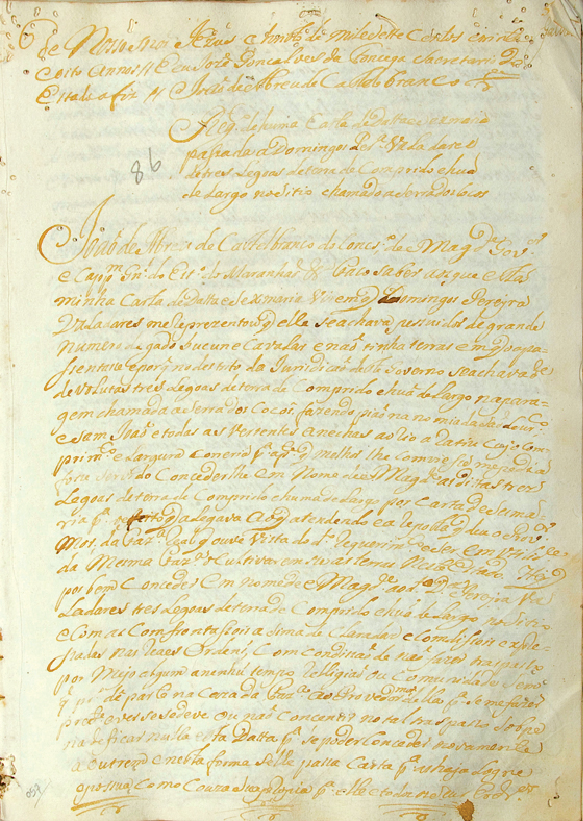
\includegraphics[width = \textwidth]
        {0167f614a7c3b3fd38127f1545dbee7c.pdf}
        \end{subfigure}
        \hspace{0.2cm}
        \qquad\tikz[baseline=-\baselineskip]\draw[ultra thick,->] (0,4) -- ++ (1,0);\qquad
        \hspace{-0.25cm}
        \begin{subfigure}[t]{0.4\textwidth}
        \centering
        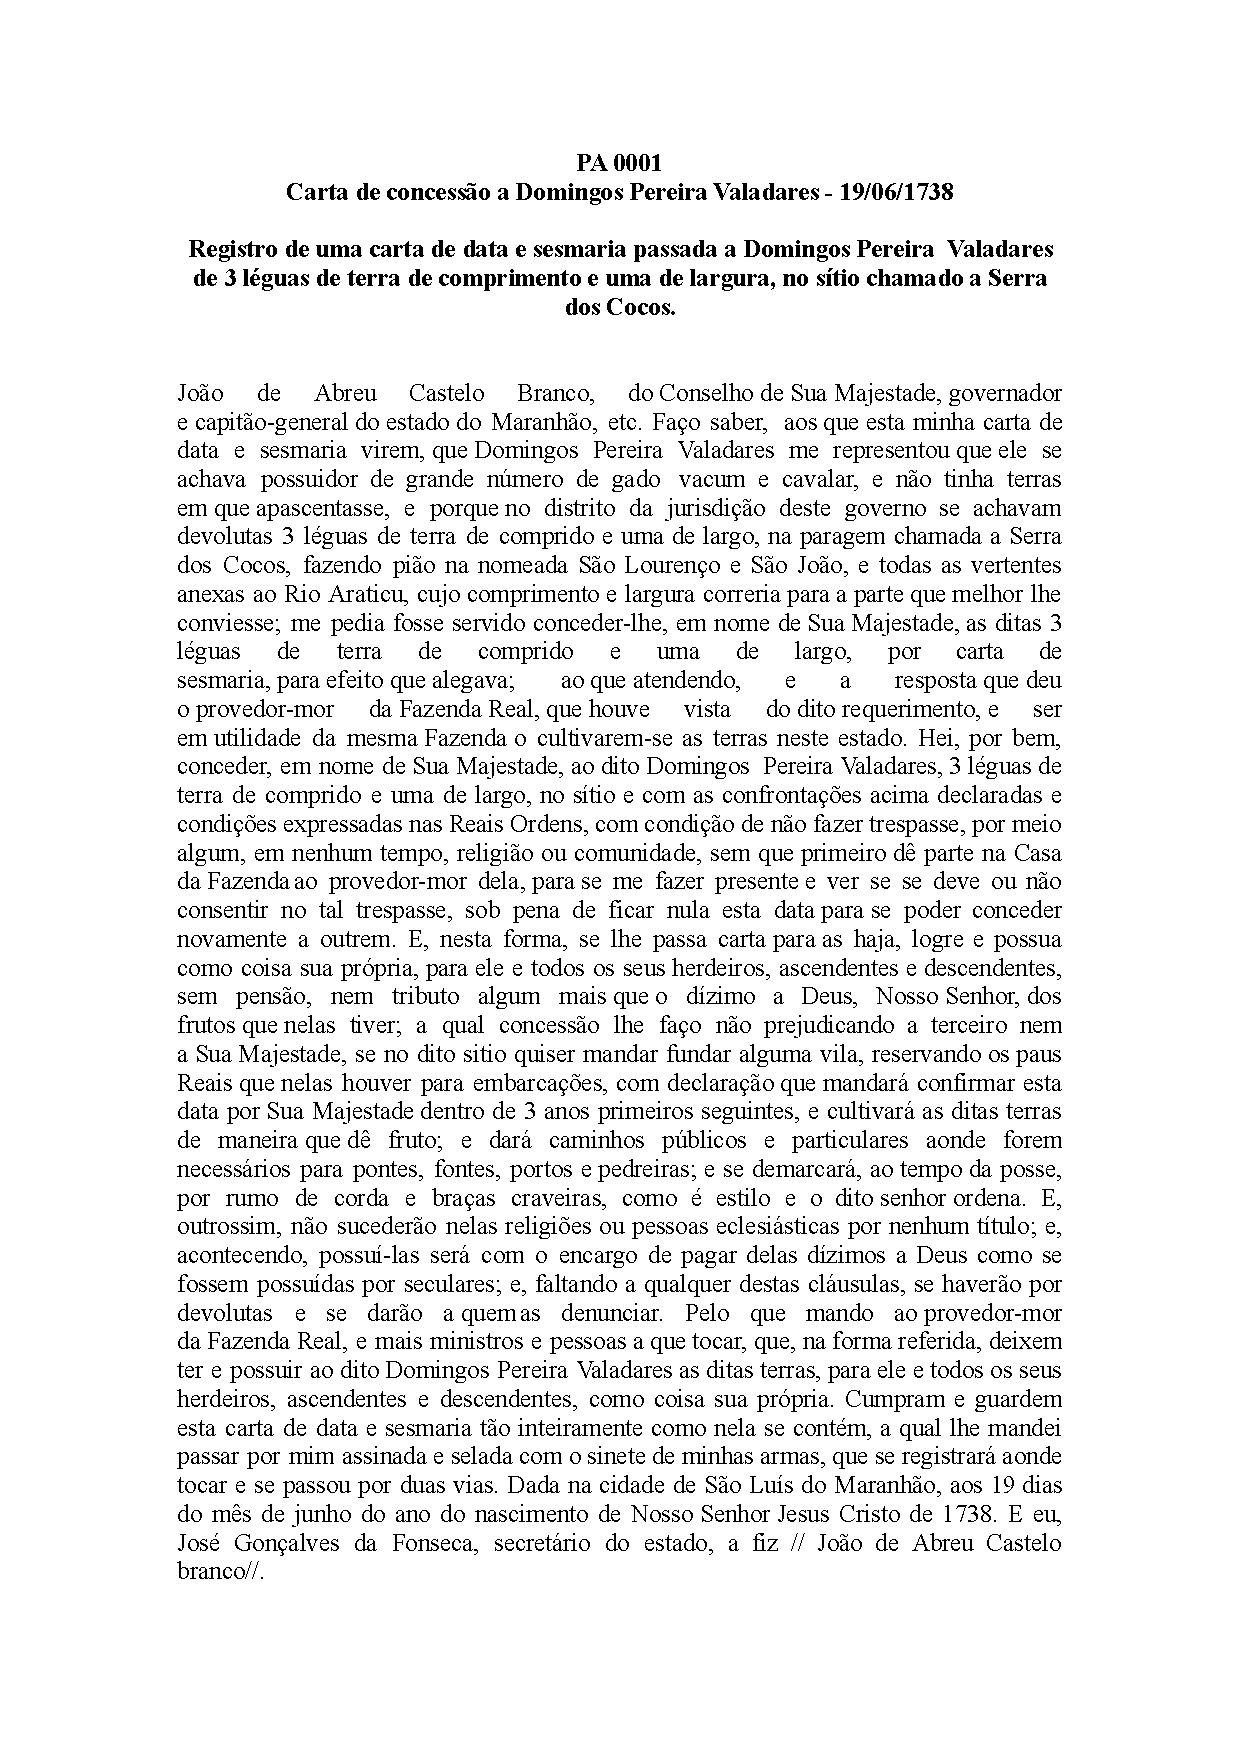
\includegraphics[page = 1, width = \textwidth]
        {ea71ea6ac7c5ec3cefa24ded60ac6438.pdf}
        \end{subfigure}
    \end{figure}
\end{frame}

% Need to create here beamer buttons so people can zoom in if they want.

% \begin{frame}{Information Extraction}
% \end{frame}

\begin{frame}{\hypertarget{data}Data}
    Information extracted from the letters:
    \begin{outline}
        \vspace{2mm}
        \1 Location.
        \vspace{2mm}
        \1 Area.
        \vspace{2mm}
        \1 What purpose was the land requested (livestock, sugar plantation/factory, etc.).
        \vspace{2mm}
        \1 Year of Concession. \hyperlink{year_dist_1697}{\beamerbutton{Size Distribution Pre and Post 1697}}
        \vspace{2mm}
        \1 Type of Settler to whom it was granted.
        \vspace{2mm}
        % \1 Concessions vs. Applications
        \1 Who granted the request.
    \end{outline}
    \vspace{2mm}
    \textbf{Summary Tables:}
    \vspace{2mm}
    \begin{outline}
        \1 Summary Tables: \hyperlink{year_2}{\beamerbutton{Municipality Summary}} \hyperlink{land_grant_level}{\beamerbutton{Land Grant Summary}}
        \vspace{2mm}
    \end{outline}
\end{frame}

\begin{frame}{Georeferenced Data}
    \centering
    \includegraphics[width=0.85\textwidth,height=0.85\textheight,keepaspectratio]
    {~/OneDrive - University of Illinois - Urbana/Research/Projects/Sesmarias Brazil/Figures/01. Maps/descriptive_map.png}
\end{frame}

% Add here the maps + the graphs I showed already. 

\begin{frame}{Treaty of Tordesillas (1494)}
    \begin{figure}
        \centering
        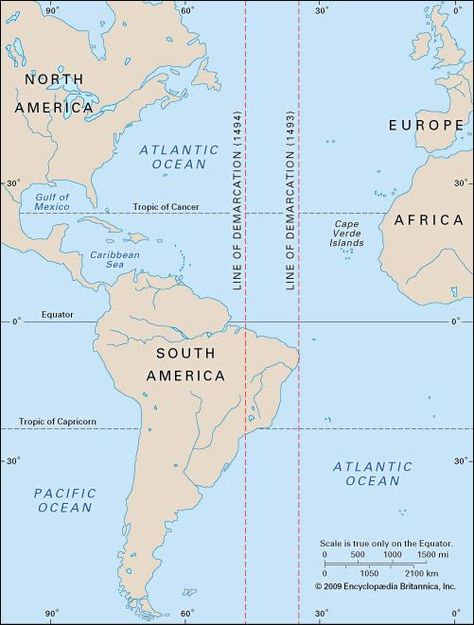
\includegraphics[width = .65\textheight]
        {treaty_tordesillas.jpeg}
        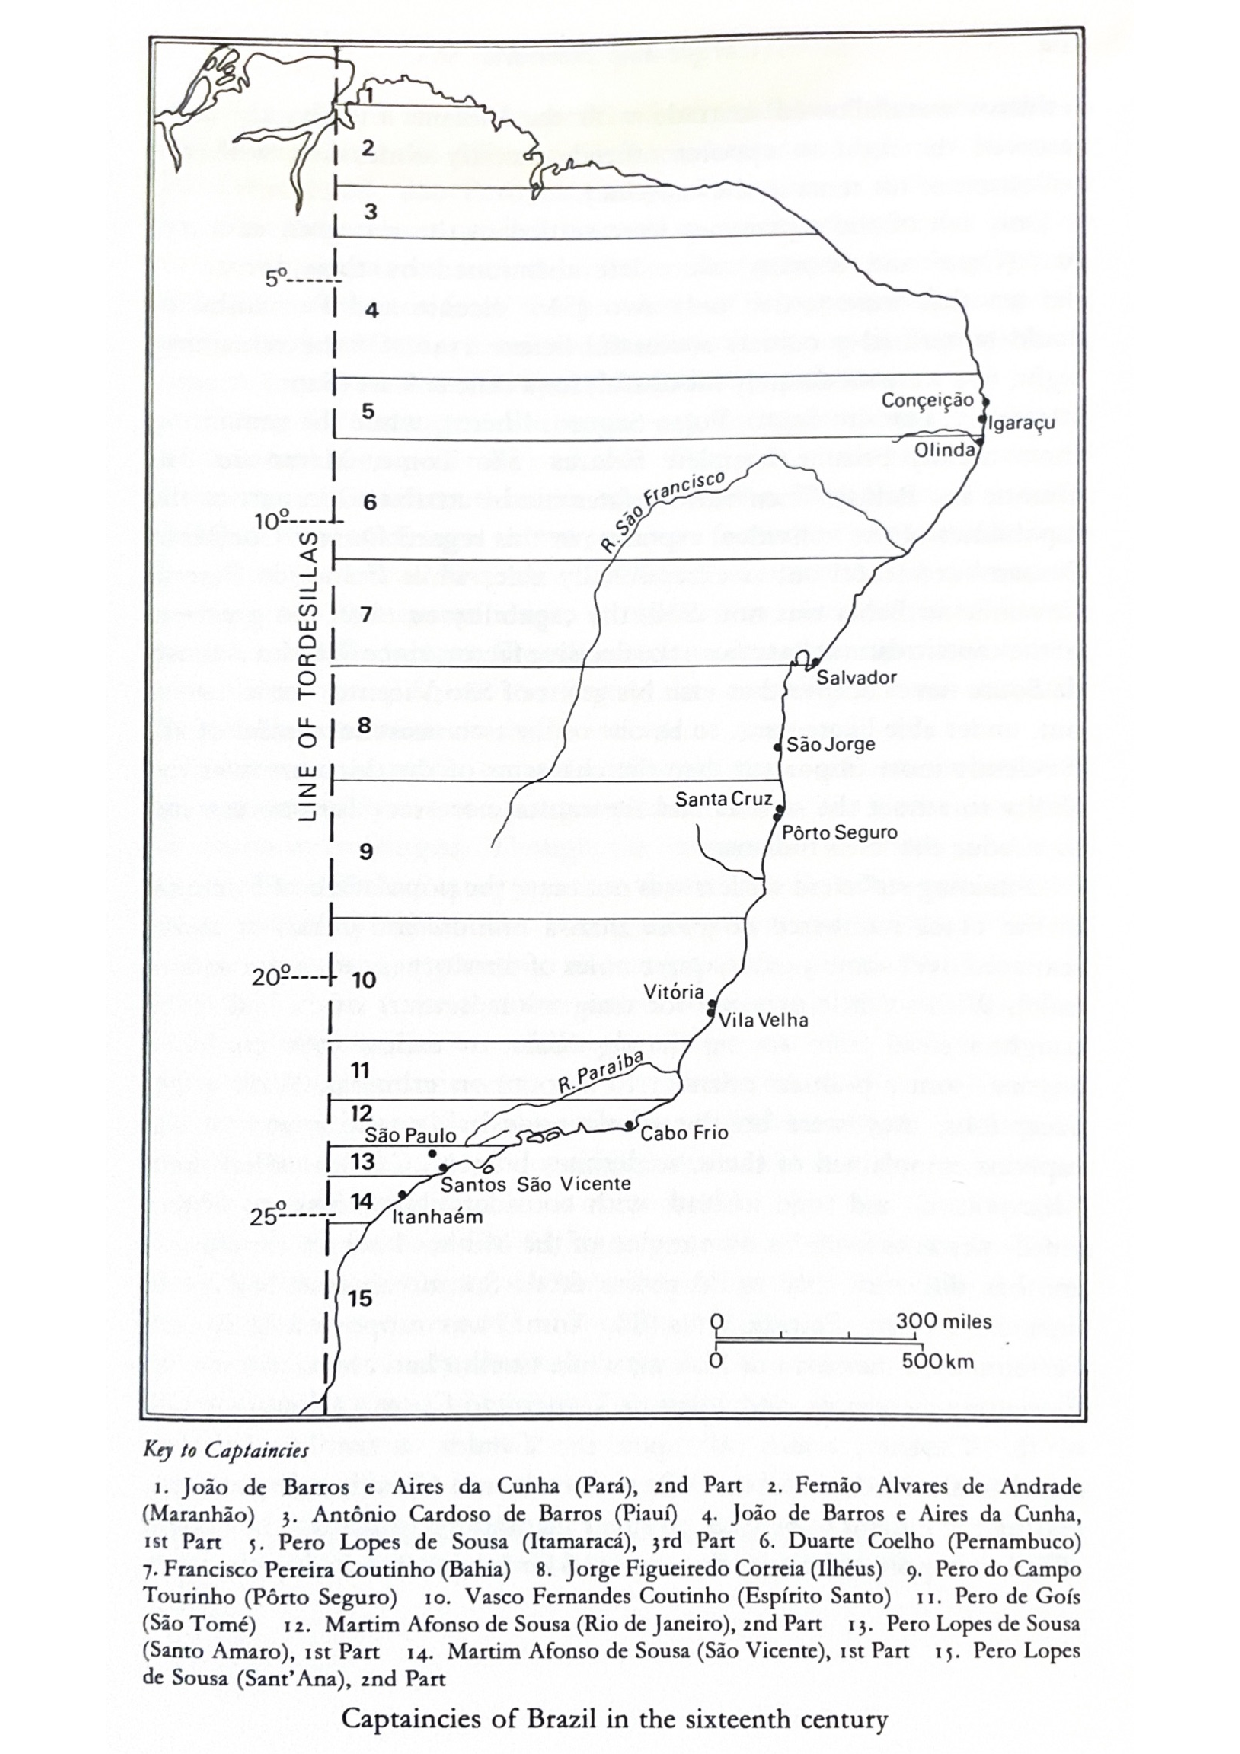
\includegraphics[width = .6\textheight]
        {bethell_tordesillas_263.pdf}
    \end{figure}
\end{frame}

\begin{frame}{Treaty of Madrid (1750)}
    \begin{figure}
        \centering
        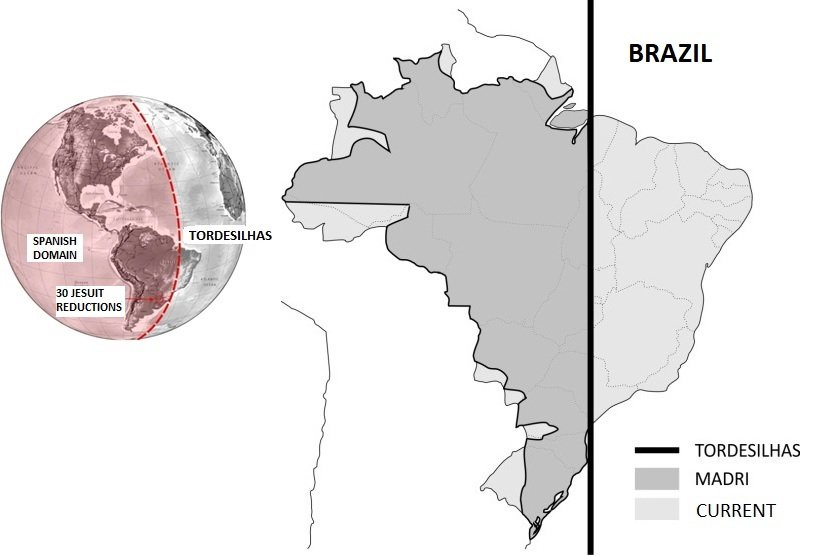
\includegraphics[width = .9\textheight]{treaty_madrid.png}
    \end{figure}
\end{frame}

\begin{frame}{Identification}{Fuzzy RDD Design}
    \begin{outline}
        \1 Estimate a Fuzzy RDD in which the probability a municipality has a land grant is a function of whether it is located to the Portuguese side of the Treaty of Tordesillas (follows \cite{Laudares2022-vy} (WP)). 
        \pause 
        \vspace{2mm}
    \end{outline}
    \vspace{2mm}
    First Stage:
    $$ LandGrant_{m,s} = \delta \cdot TT_{m,s} + f(D_{m,s})+ \mu_s + X_{m,s} + \epsilon_{m,s} $$
    Second Stage:
    $$ Y_{m,s} = \beta \cdot \widehat{LandGrant_{m,s}} + f(D_{m,s})+ \mu_s + X_{m,s} + \epsilon_{m,s}$$
    \pause 
    \begin{outline}
        \1 \textbf{Issue:} For now I only have georeferenced data along the Northeast, which would require pushing the georeferencing to states alongside the coast. Also, since a RDD would requires a lot of observations for power. 
    \end{outline}
\end{frame}

%\begin{frame}{Identification Strategy}{Standard OLS}
%    \begin{outline}
%        \1 Most basic one would be standard OLS, repeated across various censuses.
%        $$ Y_{m,s} = \beta \cdot Sesmarias_{m,s} + X_{m,s} + \mu_s + \epsilon_{m,s}$$
%            \vspace{-5mm}
%            \2 $X_{m,s}$ would contain geographical characteristics and other pre-colonial measures. 
%            \2 $Sesmarias_{m,s}$ would be a measure of the fraction of land of a municipality that was granted through a \textit{sesmaria}.
%    \end{outline}
%\end{frame}

%\begin{frame}{Identification Strategy}{Standard OLS - Heterogeneity by Grant Request}
%    \begin{outline}
%        \1 Most basic one would be standard OLS, repeated across various censuses.
%        $$ Y_{m,s} = \beta_1 \cdot Sesmarias^{ag}_{m,s} + 
%        \beta_2 \cdot Sesmarias^{lv}_{m,s} + \beta_3 \cdot Sesmarias^{mn}_{m,s} + X_{m,s} + \mu_s + \epsilon_{m,s}$$
%            \vspace{-5mm}
%            \2 $X_{m,s}$ would contain geographical characteristics and other pre-colonial measures. 
%            \2 $Sesmarias^{type}_{m,s}$ would be a measure of the fraction of land of a municipality that was granted through a \textit{sesmaria} of a certain type (agricultural, livestock, and mining).
%    \end{outline}
%\end{frame}

%\begin{frame}{Basic Descriptive Statistics}{Land History}
%    \centering
%    \includegraphics[width=0.85\textwidth,height=0.85\textheight,keepaspectratio]
%    {~/OneDrive - University of Illinois - Urbana/Research/Projects/Sesmarias Brazil/Figures/Descriptive/land_type.png}
%\end{frame}

\begin{frame}{Identification}{\cite{Dell2019-np}}
    \begin{outline}
        \1 Follow \cite{Dell2019-np} (REStud) in generating placebo land grants based on similar characteristics as the actual granted ones and estimate differential effect of both. 
        \vspace{2mm}
        \1 \textbf{Idea:} ``Propensity Score Matching'' + randomization inference, but not on unit of observation but instead on the location of the land grants
    \end{outline}
    \vspace{5mm}
    $$ Y_{i,s} = \alpha + \sum_{j = 1}^{D} \delta_1 \cdot dgrant_{i,s}^j + \beta X_{i,s} + \epsilon_{i,s}$$ 
\end{frame}

\begin{frame}{\hypertarget{IV}Identification}{Instrumental Variable}
    \begin{outline}
        \1 Exploit exogenous land quality for certain types of requests, following \cite{Wigton-Jones2020-ex} (JEG). 
    \end{outline}
    \vspace{2mm}
    First Stage:
    $$ LandGrant_{m,s} = \delta \cdot Suitability_{m,s} + \mu_s + X_{m,s} + \epsilon_{m,s} $$
    Second Stage:
    $$ Y_{m,s} = \beta \cdot \widehat{LandGrant_{m,s}} + \mu_s + X_{m,s} + \epsilon_{m,s}$$
    \pause 
    \begin{outline}
        \1 \textbf{Issue:} Tried with potential sugarcane output, and there is no first stage in 1872, but there is in 2010
        \hyperlink{sugar_table}{\beamerbutton{FS}}
        \hyperlink{sugar_table}{\beamerbutton{FS - 2010}}
    \end{outline}
\end{frame}

\begin{frame}{Descriptive Maps + OLS}\hypertarget{maps}{}
    \textbf{Descriptive:}
    \vspace{2mm}
    \begin{outline}
        \1 Description of the Land Grants: 
        \hyperlink{sugar}{\beamerbutton{Economic Activity}}  
        \hyperlink{discovery}{\beamerbutton{Discovery}} 
        \hyperlink{discovery_year}{\beamerbutton{Discovery by Year}}
        \hyperlink{no_land}{\beamerbutton{Claimed no land}}
        \hyperlink{year}{\beamerbutton{Year of Request}}
        \vspace{2mm}
        \1 1872 Census Maps: 
        \hyperlink{1872_slavery}{\beamerbutton{Slavery}}
        \hyperlink{1872_sugarcane}{\beamerbutton{Sugarcane Output}}
        \vspace{2mm}
    \end{outline}

    \vspace{2mm}
    \textbf{Grid Level:}
    \vspace{2mm}

    \begin{outline}
        \1 Sugarcane:
        \hyperlink{psugarcane_grid}{\beamerbutton{Potential Sugarcane}} 
        \hyperlink{sugarcane_grid}{\beamerbutton{Sugarcane Land Usage}} 
        \vspace{2mm}
        \1 Pasture:
        \hyperlink{pasture_grid}{\beamerbutton{Pasture Land Usage}} 
        \vspace{2mm}
        \1 Nightlight: 
        \hyperlink{nightlight_grid}{\beamerbutton{Nightlight}} 
    \end{outline}

    \vspace{2mm}
    \textbf{OLS Results:}
    \vspace{2mm}
    \begin{outline}
        \1 Land Usage: \hyperlink{econ_activities}{\beamerbutton{Economic Activity}} 
        \hyperlink{econ_dev}{\beamerbutton{Economic Development Proxies}} 
        \hyperlink{land_usage_year}{\beamerbutton{Land Usage by Year of Grant}}
    \end{outline}
\end{frame}

\begin{frame}{Future Steps}{Data Collection}
    \centering
    \includegraphics[width=0.85\textwidth,height=0.85\textheight,keepaspectratio]
    {~/OneDrive - University of Illinois - Urbana/Research/Projects/Sesmarias Brazil/Figures/01. Maps/future_step.png}
\end{frame}

\begin{frame}{Future Steps}{To Do List}
    \begin{outline}
        \1 Add more data!
        \vspace{2mm}
        \1 Add the information on the data about the people to whom the land grant was requested. 
        \vspace{2mm}
            \2 In some cases, there is some information \textbf{which city/location} the petitioner lived.
    \end{outline}
\end{frame}

\begin{frame}[allowframebreaks, t, noframenumbering, plain]{References}
    \printbibliography
\end{frame}

\appendix

\begin{frame}{History/Background}{Request Process}
    \begin{outline}
        \1 Petitioner submits a letter for an unoccupied land detailing their qualifications (captain, governor, etc.)
        \vspace{1mm}
        \pause 
        \1 Governor reads it, and if accepted returns back a letter with the requirements for the petitioner to satisfy.
        \vspace{1mm}
        \pause 
        \1 Five years to develop the land
        \vspace{1mm}
        \pause 
        \1 If successful, upon an inspection, land was transferred to the \textit{sesmeiro}.
        \vspace{1mm}
        \pause 
        \1 Able to sell, pass down as inheritance, etc. 
    \end{outline}
\end{frame}

\begin{frame}{Selection}\hypertarget{selection}{}
    \begin{outline}
        \1 Agglomeration: \hyperlink{agglomeration}{\beamerbutton{Effects on Neighboring Grids}}
    \end{outline}
\end{frame}

\begin{frame}{Identification}{Exploring the Content of the Letters}
    \begin{outline}
        \1 Focus on the letters and their contents. 
        \vspace{2mm}
        \1 Make the unit of observation a state by year. 
        \vspace{2mm}
        \1 \textbf{Example Research Question:} How would a change in state governorship affect the contents of the letter:
        \vspace{1mm}
            \2 \textbf{Channel:} New governor, not enough information on how strict he would be enforcing the land grants $\Rightarrow$ the letters are longer and more specific.
        \vspace{1mm}
    \end{outline}
\end{frame}

\begin{frame}{Other Relevant (?) Information to Add}
    \begin{outline}
        \1 \textit{Sesmarias} caused economic uncertainty in colonial times as often poor people would settle, develop land, and then lose the right of the land because a richer person would claim it \parencite[p.~142]{Da_Costa_Porto1979-dz}.
    \end{outline}
\end{frame}

\begin{frame}{Manueline Ordinances 1511-1512}
    ``Na petição por uma carta de sesmaria, o requerente devia justificar seu pedido, e quando recebesse a carta de concessão havia uma serie de obrigações entre as quais estava a necessidade do cultivo''
\end{frame}

\begin{frame}{\hypertarget{1872_slavery} 1872 Census - Slavery Distribution
    \hyperlink{maps}{\beamerbutton{Back}}} 
    
    \includegraphics[width=0.5\textwidth]
    {~/OneDrive - University of Illinois - Urbana/Research/Projects/Sesmarias Brazil/Figures/01. Maps/slave_proportion.png}
    \includegraphics[width=0.5\textwidth]
    {~/OneDrive - University of Illinois - Urbana/Research/Projects/Sesmarias Brazil/Figures/01. Maps/total_slaves.png}
\end{frame}

\begin{frame}{\hypertarget{1872_sugarcane} 1872 Census - Potential Sugarcane Output
    \hyperlink{IV}{\beamerbutton{Back}}} 
    \centering
    \includegraphics[width=0.95\textwidth]
    {~/OneDrive - University of Illinois - Urbana/Research/Projects/Sesmarias Brazil/Figures/01. Maps/sugarcane_production.png}
\end{frame}

\begin{frame}{\hypertarget{2010_sugarcane} 2010 Census - Potential Sugarcane Output
    \hyperlink{IV}{\beamerbutton{Back}}} 
    \centering
    \includegraphics[width=0.95\textwidth]
    {~/OneDrive - University of Illinois - Urbana/Research/Projects/Sesmarias Brazil/Figures/01. Maps/sugarcane_production_2010.png}
\end{frame}

\begin{frame}{\hypertarget{1872_gender} 1872 Census - Gender Distribution
    \hyperlink{maps}{\beamerbutton{Back}}} 
    %\hypertarget{1872_slavery}
    \includegraphics[width=0.5\textwidth]
    {~/OneDrive - University of Illinois - Urbana/Research/Projects/Sesmarias Brazil/Figures/01. Maps/gender_ratio.png}
    \includegraphics[width=0.5\textwidth]
    {~/OneDrive - University of Illinois - Urbana/Research/Projects/Sesmarias Brazil/Figures/01. Maps/gender_ratio_slaves.png}
\end{frame}

\begin{frame}{Basic Descriptive Statistics}
    {Year Dist. \hyperlink{maps}{\beamerbutton{Back}}}
    \centering
    \includegraphics[width=0.85\textwidth,height=0.85\textheight,keepaspectratio]
    {~/OneDrive - University of Illinois - Urbana/Research/Projects/Sesmarias Brazil/Figures/Descriptive/year_dist.png}
\end{frame}

\begin{frame}{Basic Descriptive Statistics (1 hec = 2.5 Football Fields)}
    {Size Dist. \hyperlink{maps}{\beamerbutton{Back}}} 
    \hypertarget{year_dist}
    \centering
    \includegraphics[width=0.85\textwidth,height=0.85\textheight,keepaspectratio]
    {~/OneDrive - University of Illinois - Urbana/Research/Projects/Sesmarias Brazil/Figures/Descriptive/size_dist.png}
\end{frame}

\begin{frame}{Basic Descriptive Statistics (1 hec = 2.5 Football Fields)}
    {Size Dist. \hyperlink{data}{\beamerbutton{Back}}}
    \hypertarget{year_dist_1697}
    \centering
    \includegraphics[width=0.85\textwidth,height=0.85\textheight,keepaspectratio]
    {~/OneDrive - University of Illinois - Urbana/Research/Projects/Sesmarias Brazil/Figures/Descriptive/size_dist_1697.png}
\end{frame}

\begin{frame}{Smallest Land Grant}
    \begin{outline}
        \1 The smallest land grant we have in the dataset is from 1603, in Rio de Janeiro (RJ0118). The petitioner asked for some land to build a house in the city of São Sebastião, which explains why in hectares it is so small.
    \end{outline}
\end{frame}

\begin{frame}{Basic Descriptive Statistics}{No Obs. in Pernambuco}
    \centering
    \includegraphics[width=0.85\textwidth,height=0.85\textheight,keepaspectratio]
    {~/OneDrive - University of Illinois - Urbana/Research/Projects/Sesmarias Brazil/Figures/Descriptive/year_dist_PE.png}
\end{frame}

\begin{frame}{
    \hypertarget{sugar}
    Georeferenced Land Grants
    \hyperlink{maps}{\beamerbutton{Back}}}
    {Sugarcane vs. Ranching}
    \centering
    \includegraphics[width=0.85\textwidth,height=0.85\textheight,keepaspectratio]
    {~/OneDrive - University of Illinois - Urbana/Research/Projects/Sesmarias Brazil/Figures/01. Maps/sugar_pasture.png}
\end{frame}

\begin{frame}{
    \hypertarget{discovery}
    Georeferenced Land Grants
    \hyperlink{maps}{\beamerbutton{Back}}}
    {Alleged Discovery of the Land}
    \centering
    \includegraphics[width=0.85\textwidth,height=0.85\textheight,keepaspectratio]
    {~/OneDrive - University of Illinois - Urbana/Research/Projects/Sesmarias Brazil/Figures/01. Maps/discovery.png}
\end{frame}

\begin{frame}{
    \hypertarget{discovery_year}
    Georeferenced Land Grants 
    \hyperlink{maps}{\beamerbutton{Back}}}
    {Alleged Discovery of the Land}
    \centering
    \includegraphics[width=0.85\textwidth,height=0.85\textheight,keepaspectratio]
    {~/OneDrive - University of Illinois - Urbana/Research/Projects/Sesmarias Brazil/Figures/01. Maps/discovery_year.png}
\end{frame}

\begin{frame}{
    \hypertarget{no_land}
    Georeferenced Land Grants 
    \hyperlink{maps}{\beamerbutton{Back}}}
    {Alleged Discovery of the Land}
    \centering
    \includegraphics[width=0.85\textwidth,height=0.85\textheight,keepaspectratio]
    {~/OneDrive - University of Illinois - Urbana/Research/Projects/Sesmarias Brazil/Figures/01. Maps/no_land.png}
\end{frame}

\begin{frame}{
    \hypertarget{year}
    Georeferenced Land Grants
    \hyperlink{maps}{\beamerbutton{Back}}}
    {Year of the Land Grant}
    \centering
    \includegraphics[width=0.85\textwidth,height=0.85\textheight,keepaspectratio]
    {~/OneDrive - University of Illinois - Urbana/Research/Projects/Sesmarias Brazil/Figures/01. Maps/year_distribution.png}
\end{frame}

\begin{frame}{
    \hypertarget{no_land}
    Georeferenced Land Grants 
    \hyperlink{maps}{\beamerbutton{Back}}}
    {Alleged Discovery of the Land}
    \centering
    \includegraphics[width=0.85\textwidth,height=0.85\textheight,keepaspectratio]
    {~/OneDrive - University of Illinois - Urbana/Research/Projects/Sesmarias Brazil/Figures/01. Maps/no_land.png}
\end{frame}

\begin{frame}{
    \hypertarget{no_land}
    Georeferenced Land Grants 
    \hyperlink{maps}{\beamerbutton{Back}}}
    {Alleged Discovery of the Land}
    \centering
    \includegraphics[width=0.85\textwidth,height=0.85\textheight,keepaspectratio]
    {~/OneDrive - University of Illinois - Urbana/Research/Projects/Sesmarias Brazil/Figures/01. Maps/pasture_1985_2010.png}
\end{frame}

\begin{frame}{
    \hypertarget{no_land}
    Georeferenced Land Grants 
    \hyperlink{maps}{\beamerbutton{Back}}}
    {Alleged Discovery of the Land}
    \centering
    \includegraphics[width=0.85\textwidth,height=0.85\textheight,keepaspectratio]
    {~/OneDrive - University of Illinois - Urbana/Research/Projects/Sesmarias Brazil/Figures/01. Maps/sugarcane_1985_2010.png}
\end{frame}

\begin{frame}{
    \hypertarget{no_land}
    Georeferenced Land Grants 
    \hyperlink{maps}{\beamerbutton{Back}}}
    {Alleged Discovery of the Land}
    \centering
    \includegraphics[width=0.85\textwidth,height=0.85\textheight,keepaspectratio]
    {~/OneDrive - University of Illinois - Urbana/Research/Projects/Sesmarias Brazil/Figures/01. Maps/agriculture_pasture_1985_2010.png}
\end{frame}

\begin{frame}{
    \hypertarget{no_land}
    Georeferenced Land Grants 
    \hyperlink{maps}{\beamerbutton{Back}}}
    {Alleged Discovery of the Land}
    \centering
    \includegraphics[width=0.85\textwidth,height=0.85\textheight,keepaspectratio]
    {~/OneDrive - University of Illinois - Urbana/Research/Projects/Sesmarias Brazil/Figures/01. Maps/forest_1985_2010.png}
\end{frame}

\begin{frame}{
    \hypertarget{pasture_grid}
    Georeferenced Land Grants 
    \hyperlink{grid_maps}{\beamerbutton{Back}}}
    {Pasture request + Land Usage in 2000}
    \centering
    \includegraphics[width=0.85\textwidth,height=0.85\textheight,keepaspectratio]
    {~/OneDrive - University of Illinois - Urbana/Research/Projects/Sesmarias Brazil/Figures/01. Maps/pasture_2000_grid.png}
\end{frame}

\begin{frame}{
    \hypertarget{psugarcane_grid}
    Georeferenced Land Grants 
    \hyperlink{maps}{\beamerbutton{Back}}}
    {Sugarcane request + Potential Sugarcane Production}
    \centering
    \includegraphics[width=0.85\textwidth,height=0.85\textheight,keepaspectratio]
    {~/OneDrive - University of Illinois - Urbana/Research/Projects/Sesmarias Brazil/Figures/01. Maps/sugarcane_potential_2000_grid.png}
\end{frame}

\begin{frame}{
    \hypertarget{sugarcane_grid}
    Georeferenced Land Grants 
    \hyperlink{maps}{\beamerbutton{Back}}}
    {Sugarcane request + Area used for Sugarcane (2000)}
    \centering
    \includegraphics[width=0.85\textwidth,height=0.85\textheight,keepaspectratio]
    {~/OneDrive - University of Illinois - Urbana/Research/Projects/Sesmarias Brazil/Figures/01. Maps/sugarcane_usage_2000_grid.png}
\end{frame}

\begin{frame}{
    \hypertarget{nightlight_grid}
    Georeferenced Land Grants 
    \hyperlink{maps}{\beamerbutton{Back}}}
    {All requests + Nightlight data (2000)}
    \centering
    \includegraphics[width=0.85\textwidth,height=0.85\textheight,keepaspectratio]
    {~/OneDrive - University of Illinois - Urbana/Research/Projects/Sesmarias Brazil/Figures/01. Maps/nightlight_2000_grid.png}
\end{frame}


\begin{frame}{
    \hypertarget{sugar_table}
    First-Stage Estimates - 1872 
    \hyperlink{IV}{\beamerbutton{Back}}}
    \centering
    \input{~/OneDrive - University of Illinois - Urbana/Research/Projects/Sesmarias Brazil/Tables/sugar_first_stage.tex}
\end{frame}

\begin{frame}{
    \hypertarget{sugar_table_2010}
    First-Stage Estimates - 2010
    \hyperlink{IV}{\beamerbutton{Back}}}
    \centering
    \input{~/OneDrive - University of Illinois - Urbana/Research/Projects/Sesmarias Brazil/Tables/sugar_first_stage_2010.tex}
\end{frame}

\begin{frame}{
    \hypertarget{sugar_table_2010}
    First-Stage Estimates - Grid
    \hyperlink{IV}{\beamerbutton{Back}}}
    \centering
    \input{~/OneDrive - University of Illinois - Urbana/Research/Projects/Sesmarias Brazil/Tables/sugar_first_stage_grid.tex}
\end{frame}

\begin{frame}{
    \hypertarget{econ_activities}
    OLS - Economic Activities
    \hyperlink{maps}{\beamerbutton{Back}}}
    \centering
    \input{~/OneDrive - University of Illinois - Urbana/Research/Projects/Sesmarias Brazil/Tables/economic_activity_grid.tex}
\end{frame}

\begin{frame}{
    \hypertarget{econ_dev}
    OLS - Economic Development
    \hyperlink{maps}{\beamerbutton{Back}}}
    \centering
    \input{~/OneDrive - University of Illinois - Urbana/Research/Projects/Sesmarias Brazil/Tables/economic_development_grid.tex}
\end{frame}

\begin{frame}{
    \hypertarget{land_usage_year}
    OLS - Land Usage
    \hyperlink{maps}{\beamerbutton{Back}}}
    \centering
    \input{~/OneDrive - University of Illinois - Urbana/Research/Projects/Sesmarias Brazil/Tables/land_usage_year_grid.tex}
\end{frame}

\begin{frame}{
    \hypertarget{agglomeration}
    OLS - Agglomeration
    \hyperlink{selection}{\beamerbutton{Back}}}
    \centering
    \input{~/OneDrive - University of Illinois - Urbana/Research/Projects/Sesmarias Brazil/Tables/agglomeration_grid.tex}
\end{frame}

\begin{frame}
    {Balance Tables \hyperlink{data}{\beamerbutton{Back}}}
    \hypertarget{grid_balance}
    {Grid Level}
    \begin{center}
    \input{~/OneDrive - University of Illinois - Urbana/Research/Projects/Sesmarias Brazil/Tables/summary_sesmarias_grid.tex}
    \end{center}
\end{frame}

\begin{frame}[shrink=25]{
    \hypertarget{year_2}
    Balance Tables 
    \hyperlink{data}{\beamerbutton{Back}}}
    {1872 Municipality Level}
    \begin{center}
    \input{~/OneDrive - University of Illinois - Urbana/Research/Projects/Sesmarias Brazil/Tables/summary_1872.tex}
    \end{center}
\end{frame}

\begin{frame}{
    \hypertarget{land_grant_level}
    Balance Tables 
    \hyperlink{data}{\beamerbutton{Back}}}
    {\textcolor{white}{Land Grant Level}}
    \centering
    \input{~/OneDrive - University of Illinois - Urbana/Research/Projects/Sesmarias Brazil/Tables/summary_sesmarias.tex}
\end{frame}

\end{document}